%
% slides.tex
%
% (c) 2019 Prof Dr Andreas Müller, Hochschule Rapperswil
%

\ifthenelse{\boolean{presentation}}{
\begin{frame}
\titlepage
\end{frame}
}{}

%
%
%
\begin{frame}
\frametitle{Aufgabenstellung}
\begin{block}{Aufgabe}
Finde $h_k$ derart, dass die Funktion $\varphi$ kompakten Träger hat.
\end{block}
\uncover<2->{
\begin{block}{Forderungen}
\begin{enumerate}
\item<2-> Skalierungsrelation 
\[
\varphi(t) = \sqrt{2} \sum_{k\in\mathbb Z} h_k \varphi(2t-k)
\qquad\Leftrightarrow\qquad
\hat{\varphi}(\omega)
=
H\biggl(\frac{\omega}2\biggr)
\hat{\varphi}\biggl(\frac{\omega}2\biggr)
\]
\item<3->
``schön''
\end{enumerate}
\end{block}
}
\end{frame}

%
% Algebraische Aufgabenstellung
%
\begin{frame}
\frametitle{Algebraische Aufgabe}

\begin{block}{Aufgabe}
Finde ein trigonometrisches Polynome
\[
H(\omega) = \frac{1}{\sqrt{2}}\sum_{k\in\mathbb Z} h_ke^{-ik\omega}
\]
derart, dass
\begin{enumerate}
\item $H(0)=1$
\item $|H(\omega)|^2+|H(\omega+\pi)|^2 = 1$
\end{enumerate}
\end{block}

\begin{block}{Haar-Lösung}
\[
H_{\text{Haar}}(\omega) = \frac12(1+e^{-i\omega})
\qquad\Rightarrow\qquad
h_0=h_1=\frac1{\sqrt{2}}
\]
\end{block}

\end{frame}

%
% 
%
\begin{frame}
\frametitle{Zusatzforderung: reell}
\begin{block}{Forderung}
Reale Signale spielen sich in $\mathbb R$ ab: $\varphi$ soll reellwertig
sein.
\end{block}
$\Rightarrow$ $h_k\in\mathbb R$

\uncover<2->{
\[
\overline{H(\omega)}
=
\frac{1}{\sqrt{2}} \sum_{k\in\mathbb Z} \overline{\mathstrut h_k}\; \overline{e^{-i\omega k}}
=
\frac{1}{\sqrt{2}} \sum_{k\in\mathbb Z} 
h_k e^{i\omega k}
}
\uncover<3->{=
H(-\omega)
}
\]

\end{frame}

%
% Glattheit
%
\begin{frame}
\frametitle{Zusatzforderung: Ordnung}
\begin{definition}
Das Wavelet $\psi$ hat die Ordnung $N$, wenn $t^N\psi\in L^1(\mathbb R)$ und
\[
\int t^k \psi(t)\,dt = 0 \text{ für $k<N$}
\]
\end{definition}
\begin{block}{Forderung}
$\psi$ soll möglichst hohe Ordnung haben.
\end{block}
\end{frame}

%
% Konsequenz der Ordnungsforderung
%
\begin{frame}
\frametitle{Konsequenz}
\begin{block}{Ableitungen von $\hat{\psi}$}
%\vspace{-20pt}
\begin{align*}
\frac{d}{d\omega} \hat{\psi}(\omega)
&\uncover<2->{=
\frac{d}{dt}
\frac{1}{\sqrt{2\pi}}
\int \psi(t)e^{-i\omega t}\,dt}
\uncover<3->{=
(-i)
\frac{1}{\sqrt{2\pi}}
\int
t
\psi(t)e^{-i\omega t}\,dt}
\\
\uncover<4->{\frac{d^k}{d\omega^k} \hat{\psi}(\omega)}
&\uncover<5->{=
(-i)^k
\frac{1}{\sqrt{2\pi}}
\int
t^k
\psi(t)e^{-i\omega t}\,dt}
\end{align*}
\uncover<6->{Hohe Ordnung von $\psi$}
\uncover<7->{$\Leftrightarrow$
hohe ``Glattheit'' von
$\hat{\psi}$ 
bei $\omega=0$}
\end{block}
%\vspace{-10pt}
\uncover<8->{
\begin{block}{$\psi$ von Ordnung $N$}
\[
\frac{d^k}{d\omega^k}
\hat{\psi}(0) = (-i)^k \frac{1}{\sqrt{2}} \int t^k \psi(t)\,dt = 0
\text{ für $k < N$}
\]
\end{block}
}
\end{frame}


\begin{frame}
\frametitle{Konsequenz}
\begin{block}{Taylor-Reihe von $\hat{\psi}$}
\[
\hat{\psi}(\omega)
\uncover<2->{
= \frac{1}{N!}\hat{\psi}^{(N)}(0)\cdot\omega^N
+\text{Terme höherer Ordnung}
}
\]
\end{block}
\uncover<3->{%
$\Rightarrow$ $\hat{\psi}$ hat Nullstelle $N$-ter Ordnung bei $\psi$}
\uncover<4->{%
\[
\hat{\psi}(\omega)
=
e^{i\omega/2}
\overline{H\biggl(\frac{\omega}2+\pi\biggr)}
\hat{\varphi}\biggl(\frac{\omega}2\biggr)
\]
}
\uncover<5->{$\Rightarrow$ $H(\omega)$ hat eine Nullstelle $N$-ter Ordnung bei $\omega=\pi$}

\end{frame}

%
% Nullstelle herausfaktorisieren
%
\begin{frame}
\frametitle{Nullstelle Herausfaktorisieren}
\begin{block}{Reine Nullstelle}
\begin{align*}
\biggl(\frac{1+e^{-i\omega}}{2}\biggr)^{\phantom{N}}
&\quad\text{hat einfache Nullstelle bei $\omega=\pi$}
\\
\uncover<2->{\biggl(\frac{1+e^{-i\omega}}{2}\biggr)^N}
&\quad\uncover<2->{\text{hat $N$-fache Nullstelle bei $\omega=\pi$}}
\end{align*}
\end{block}
\uncover<3->{
\begin{block}{Faktorisieren}
\[
H(\omega)
=
\biggl(\frac{1+e^{-i\omega}}{2}\biggr)^N
B(\omega)
\]
trigonometrisches Polynom%
\uncover<4->{, $B(\omega)$ hat keine Nullstelle bei $\omega=\pi$}
\end{block}
}
\end{frame}

%
% Betrag
%
\begin{frame}
\frametitle{Betrag}
\begin{block}{Betrag $M(\omega)$}
\[
M(\omega) = |H(\omega)|^2 = H(\omega)H(-\omega)
\]
$M(\omega)$ ist gerade\uncover<2->{, also ein Polynom in $\cos\omega$}
\end{block}
\uncover<3->{
\begin{block}{Faktorisierung}
$M(\omega)$ enthält den Faktor
\[
\biggl(\frac{1+e^{-i\omega}}2\biggr)^N
\biggl(\frac{1+e^{+i\omega}}2\biggr)^N
\ifthenelse{\boolean{presentation}}{
\only<4>{=\biggl(\frac{1+2\cos\omega+1}4\biggr)^N
}}{}
\only<5->{=
\biggl(\frac{1+\cos\omega}2\biggr)^N}
\uncover<6->{=
\biggl(\cos^2\frac{\omega}2\biggr)^N
}
\]
\uncover<7->{Daher
\[
M(\omega)
\uncover<7->{=
\biggl(\cos^2\frac{\omega}2\biggr)^N A(\omega)}\uncover<8->{,\quad
A(\omega)=B(\omega)B(-\omega)}
\uncover<9->{=
\tilde{P}(\cos\omega)}
\]
}
\end{block}
}
\end{frame}

%
% Gleichung für P
%
\begin{frame}
\frametitle{Neue Variable}
\begin{block}{Schreibe $y=\sin^2\frac{\omega}2$}
\vspace{-20pt}
\begin{align}
&\uncover<1->{\Rightarrow}&
\uncover<1->{1-y}&\uncover<1->{= \cos^2\frac{\omega}2}
\notag
\\
&\uncover<2->{\Rightarrow}&
\uncover<2->{A(\omega)}&\uncover<2->{=\tilde{P}(\cos\omega)=\tilde{P}(1-2y)=:P(y)}
\notag
\\
&\uncover<3->{\Rightarrow}&
\uncover<3->{M(\omega)}&\uncover<3->{=(1-y)^N P(y)}
\notag
\\
&\uncover<4->{\Rightarrow}&
\uncover<4->{\cos^2\frac{\omega+\pi}2}&\uncover<4->{=\sin^2\frac{\omega}2=y}
\notag
\\
&\uncover<5->{\Rightarrow}&
\uncover<5->{M(\omega)+M(\omega+\pi)}&\uncover<5->{= (1-y)^N P(y) + y^N P(1-y) = 1}
\label{algcond}
\end{align}
\uncover<6->{%
Problem reduziert auf das algebraische Problem, ein Polynom $P$ zu finden,
welches die Gleichung~\eqref{algcond} erfüllt.
}
\end{block}
\end{frame}

%
%
%
\begin{frame}
\frametitle{Lösung}
\begin{block}{Partialbruchzerlegung}
\[
\frac{1}{y^N(1-y)^N}
\uncover<2->{=
\sum_{k=1}^N \frac{\mathstrut C_k}{\mathstrut y^k}
+
\sum_{k=1}^N \frac{\mathstrut C_k'}{\mathstrut (1-y)^k}
}
\]
\uncover<3->{Symmetrie: }\uncover<4->{$C_k'=C_k$}
\end{block}
\[
\uncover<5->{P_N(y) = \sum_{k=1}^N C_ky^{N-k}}
\]
\uncover<6->{erfüllt}
\[
\uncover<7->{1=
P_N(y) (1-y)^N + y^N P_N(1-y)}
\]
\uncover<8->{%
$\Rightarrow$ Für jedes $N$ gibt es ein geeignetes Polynom.}
\end{frame}

%
% Fallunterscheidung
%
\begin{frame}
%\frametitle{Fallunterscheidung}
\begin{center}
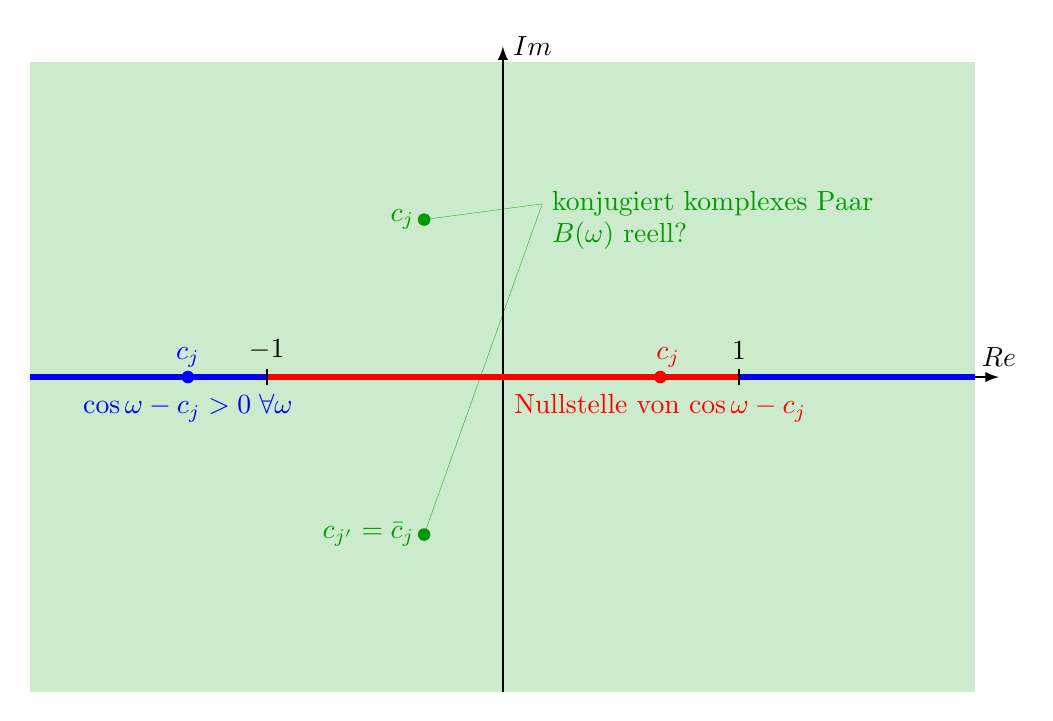
\begin{tikzpicture}[>=latex]
\definecolor{darkgreen}{rgb}{0,0.6,0}
\fill[color=darkgreen!20] (-6,-4) rectangle (6,4);
\fill[color=darkgreen] (-1,2) circle[radius=0.08];
\fill[color=darkgreen] (-1,-2) circle[radius=0.08];
\node[color=darkgreen] at (0.5,2.2) [right] {konjugiert~komplexes Paar};
\node[color=darkgreen] at (0.5,1.8) [right] {$B(\omega)$ reell?};
\draw[line width=0.1pt,color=darkgreen] (-1,2)--(0.5,2.2);
\draw[line width=0.1pt,color=darkgreen] (-1,-2)--(0.5,2.2);
\node[color=darkgreen] at (-1,2) [left] {$c_j$};
\node[color=darkgreen] at (-1,-2) [left] {$c_{j'}=\bar{c}_j$};
\draw[->,line width=0.7pt] (-6,0)--(6.3,0)
	coordinate[label={$\operatorname{Re}$}];
\draw[->,line width=0.7pt] (0,-4)--(0,4.2)
	coordinate[label={right:$\operatorname{Im}$}];
\draw[color=red,line width=2pt] (-3,0)--(3,0);
\draw[color=blue,line width=2pt] (3,0)--(6,0);
\draw[color=blue,line width=2pt] (-3,0)--(-6,0);
\fill[color=blue] (-4,0) circle[radius=0.08];
\node[color=blue] at (-4,0) [above] {$c_j$};
\node[color=blue] at (-4,-0.1) [below] {$\cos\omega -c_j>0\;\forall\omega$};
\node[color=red] at (2.1,0) [above] {$c_j$};
\fill[color=red] (2,0) circle[radius=0.08];
\node[color=red] at (2,-0.1) [below] {Nullstelle von $\cos\omega - c_j$};
\node at (3,0.1) [above] {$1$};
\draw[line width=0.7pt] (-3,-0.1)--(-3,0.1);
\node at (-3,0.1) [above] {$-1$};
\draw[line width=0.7pt] (3,-0.1)--(3,0.1);
\end{tikzpicture}
\end{center}
\end{frame}

\begin{frame}
\frametitle{Hilfsformel}
\begin{align*}
\frac{z+z^{-1}}2 - \frac{s+s^{-1}}2
&=
-\frac{1}{2s} (z-s)(z^{-1}-s)
\\
\cos\omega - \frac{s+s^{-1}}2
&=
-\frac{1}{2s} (e^{-i\omega}-s)(e^{i\omega}-s)
\\[10pt]
A_j(\omega)=\cos\omega-c_j&=B_j(\omega)B_j(-\omega)
\end{align*}
\end{frame}
